\documentclass[aspectratio=169,usenames,dvipsnames]{beamer}
\beamertemplatenavigationsymbolsempty
% \documentclass{beamer}

% UNCOMMENT FOR HANDOUTS
% \usepackage{pgfpages}
% \pgfpagesuselayout{2 on 1}[landscape,letterpaper,border shrink=5mm]
% \setbeameroption{show notes}

\mode<presentation>
\usetheme{Boadilla}
\usecolortheme{spruce}
\usepackage{../../LizStyle,ulem}
\usepackage{color}
\usepackage[color,matrix,arrow]{xy}
% \input xy
% \xyoption{all}
\usepackage{tikz}
\usepackage{tikz-cd}
\tikzset{commutative diagrams/diagrams={ampersand replacement=\&}}

\AtBeginSection{\frame{\sectionpage}}


% ==========Command for putting comments and removing them=======
% Visible:
\newcommand{\InstructorNotes}[1]{\textit{\color{orange}#1}}
\newcommand{\InstructorList}[1]{
\begin{itemize}
	\color{orange}
	#1
\end{itemize}
}
% Removed:
\renewcommand{\InstructorNotes}[1]{}
\renewcommand{\InstructorList}[1]{}


\newcommand{\bvfill}{\vskip0pt plus 1filll}

\usepackage{multimedia}
\usepackage{graphbox}

% \usepackage{algpseudocode}


\newcommand{\Reeb}{\textbf{Reeb}}
\newcommand{\Rtopc}{\textbf{Rtopc}}
% \newcommand{\RR}{\mathcal{R}}

\newcommand{\Set}{\textbf{Set}}
\newcommand{\Vect}{\textbf{Vect}}
\newcommand{\Top}{\textbf{Top}}
\newcommand{\Int}{\textbf{Int}}


\graphicspath{ {Figures/} {../Figures/}{../../Figures/} }



\begin{document}
%\pdfoptionpdfminorversion 5
%\logo{\includegraphics[height=1.5cm]{dukeshield.pdf}}
\title[]{Ch 7.1-7.2: Polynomial regression and Step Functions}
\subtitle{Lecture 21 - CMSE 381}
\date{Wed, Mar 18, 2026}



\institute[MSU-CMSE]{Michigan State University\\
			::\\
          Dept of Computational Mathematics, Science \& Engineering}
%\author[Dr.~Zhang]{Prof.~Mengsen Zhang}

\begin{frame}
 \titlepage


\end{frame}
%--------------------------
\begin{frame}[c]{Announcements}

\begin{columns}
\column{.45\textwidth}
\centering

	\textbf{Last time:}
	\begin{itemize}
		\item Exam 2
	\end{itemize}

	\vspace{.2in}

	\textbf{This lecture:}
	\begin{itemize}
	\item 7.1 Polynomial regression
	\item 7.2 Step functions
\end{itemize}
\centering

\textbf{Announcements:}
	\begin{itemize}
		\item HW \#5 due Sun 3/29
		\item Project stuff

	\end{itemize}


\column{.45\textwidth}
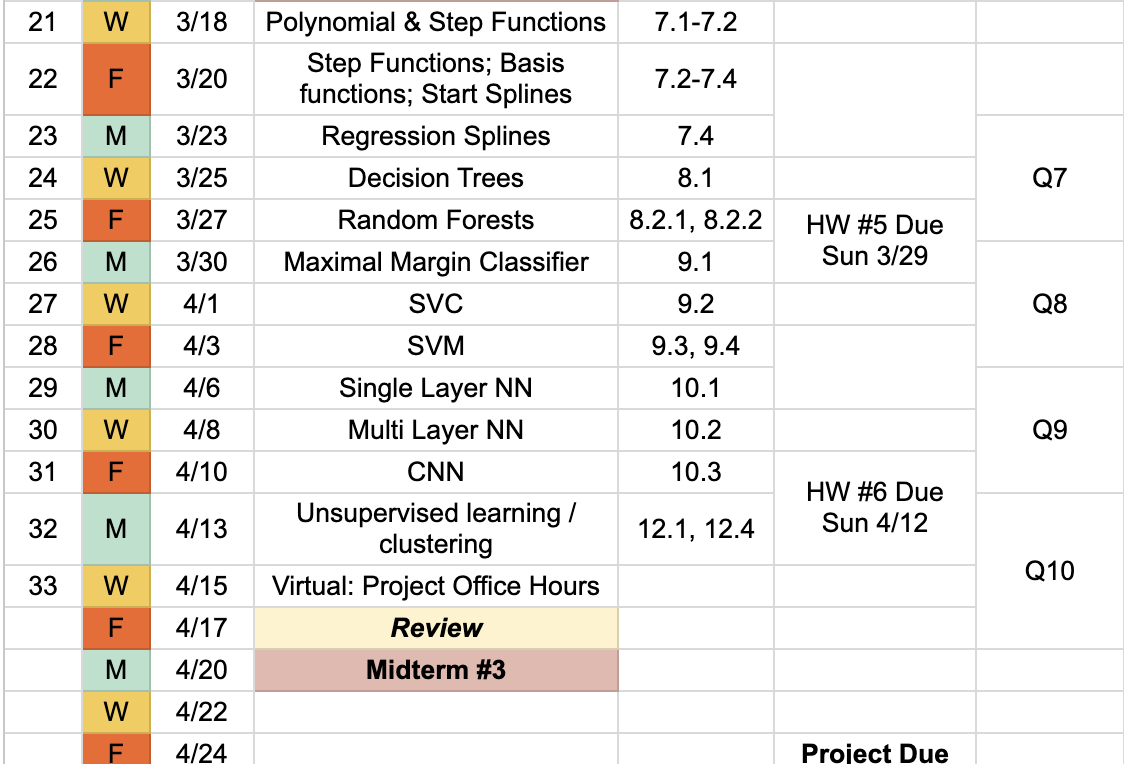
\includegraphics[width = \textwidth]{Schedule-S26-3.png}
\end{columns}

\end{frame}

\begin{frame}[c]{What should you learn from today's lecture?}
	\begin{itemize}
		\item Why do people want to use polynomial regression rather than simple linear regression
		\item How to fit polynomial regression models?
		\item Why do people want to use step functions rather than simple linear regression?
		\item How to fit step function models? 
		\item What is common between polynomial regression and step functions?
		\item What is different between polynomial regression and step functions?
	\end{itemize}
\end{frame}
%--- Next Frame ---%



% %=================
% \section{Last time}
% %=================



% \begin{frame}[t]{High-Dimensional Data}

% \begin{columns}
% \column{.45\textwidth}
% \centering
% \textbf{Low-Dimensions}

% $n \gg p$

% \footnotesize
% \begin{itemize}
% \item Low here means $p$ is low, or at least small relative to $n$
% \item Can do all the stuff we've talked about so far
% \end{itemize}
% \column{.45\textwidth}
% \centering
% \textbf{High-Dimensions}

% $n \ll p$

% \footnotesize
% \begin{itemize}
% 	\item Issues show up even if $p$ is close to or slightly smaller than $n$
% 	\item Classical approaches not appropriate since lots of overfitting
% \end{itemize}



% \end{columns}
% \bvfill
% \centering
% \textbf{What to do about it?}

% Be less flexible....
% \bvfill
% \end{frame}
% %--- Next Frame ---%


% %--- Next Frame ---%
% %--- Next Frame ---%
% \begin{frame}[t]{Key points }

% \begin{columns}
% \column{.45\textwidth}
% \centering

% \begin{itemize}
%   \item regularization
% or shrinkage plays a key role in high-dimensional problems, \item  appropriate
% tuning parameter selection is crucial for good predictive performance, and
% \item  the test error tends to increase as the dimensionality of the problem increases, unless the additional
% features are truly associated with the response.
% \end{itemize}

% \column{.45\textwidth}
% \centering
% \begin{itemize}
% 	\item Curse of dimensionality
%   \item Report results on an independent test set, or cross-validation errors.
  
% \end{itemize}
% \InstructorNotes{Prior stuff for reducing flexibility. Next chapter is for increasing flexibility}
% \end{columns}

% \end{frame}
% %--- Next Frame ---%


%==========
\section{Polynomial Regression}
%==========

\begin{frame}[c]{Polynomial regression}

\begin{columns}
\column{.45\textwidth}
\centering
Replace linear model
\begin{equation*}
	y_i = \beta_0 + \beta_1x_1 + \e_i
\end{equation*}
with
\begin{equation*}
	y_i = \beta_0 + \beta_1x_1 + \beta_2x_i^2 + \cdots + \beta_dx_i^d + \e_i
\end{equation*}

\column{.45\textwidth}
\centering
\InstructorList{
  \item Can learn with linear models by passing in predictors $x_i^\ell$
	\item Tend to not go higher than degree 3 or 4 because makes overly flexible
}

\end{columns}

\end{frame}
%--- Next Frame ---%
\begin{frame}[t]{Example: Wage Data}

	$$
\texttt{wage} = \beta_0 + \beta_1 \texttt{age} + \beta_2 \texttt{age}^2 + \cdots + \beta_p \texttt{age}^p +\varepsilon.
$$

   My code learned:
  $$
  -184.1542 + 21.24552 \cdot age + -0.56386 \cdot age^2 + 0.00681 \cdot age^3 + (-3\cdot 10^{-5}) \cdot age^4
  $$

\begin{columns}
\column{.45\textwidth}
\centering

\InstructorList{
	\item Make a matrix of predictors $X$ with columns $X^0, X^1, X^2, \cdots, X^p$
	\item Then can use linear regression to learn the coefficients
}
	
\column{.45\textwidth}
\centering
\InstructorList{
  \item Plot of wage vs age for men in central Atlantic region of the US
  \item Equivalent figure from the book on the next page
}
\end{columns}

\end{frame}
%--- Next Frame ---%

\begin{frame}[c]{Example with wage data}

\begin{columns}
\column{.45\textwidth}
\centering
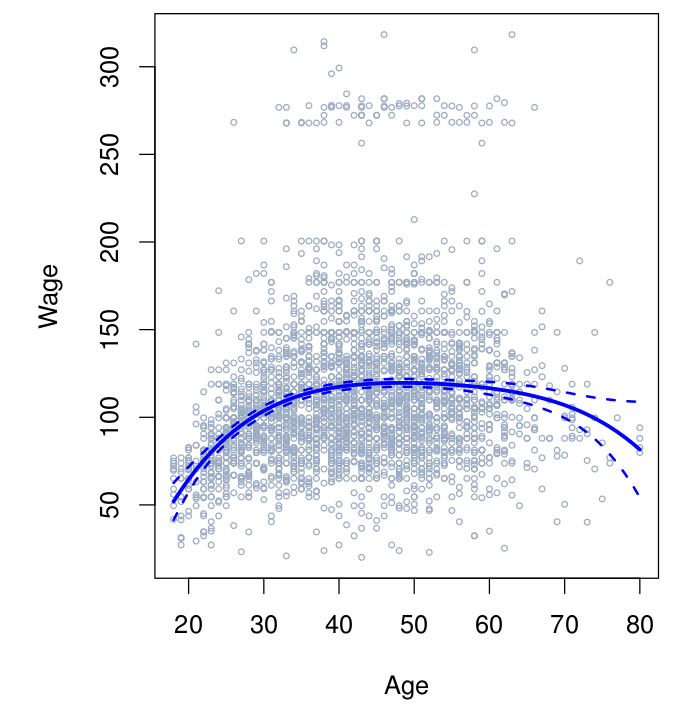
\includegraphics[width = \textwidth, align = c]{Fig7-1a}

\column{.45\textwidth}
\centering
\InstructorList{
	\item Dark line is degree 4 polynomial
	\item Have variance for each coefficient
	\item Assume you have a model $\hat f(x_0) = \hat \beta_0 + \hat \beta_1 x_0 + \cdots + \hat \beta_d x_0^d$
	\item Can use that to estimate the pointwise variance $\Var(\hat f(x_0))$
	\item Draw 2 std deviations away from the line, 95\% confidence interval
}

\end{columns}

\end{frame}
%--- Next Frame ---%

%==========
\section{Step function}
%==========



\begin{frame}[t]{Step functions}
\begin{equation*}
	\mathrm{I}(X < c) \qquad \mathrm{I}(c_1 \leq X < c_2) \qquad \mathrm{I} (c \leq X)
\end{equation*}
\begin{columns}
\column{.45\textwidth}
\centering
\InstructorList{
 \item Draw each of the functions above
}

\column{.45\textwidth}
\centering

\end{columns}

\end{frame}
%--- Next Frame ---%
\begin{frame}[c]{More on step function setup}

\begin{columns}
\column{.45\textwidth}
\centering
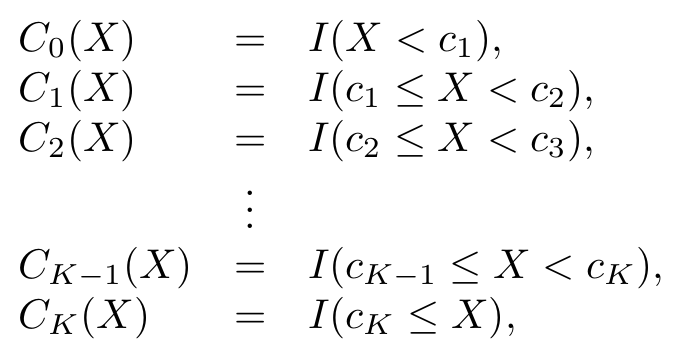
\includegraphics[width = \textwidth, align = c]{Eq7-4}
\vfill



\column{.45\textwidth}
\centering
\InstructorList{
 \item Choose values $c_1,\cdots, c_K$
  \item Allow to learn models that don't have global structure
	\item Use indicator functions to break up the range of $X$ into bins, then we can fit a new constant in each bin.
	\item these are sometimes also called dummy variables
	\item Note that $\sum_j C_j(X) = 1$ because $X$ is in only one interval
}

\end{columns}

\end{frame}
%--- Next Frame ---%
{
\setbeamercolor{background canvas}{bg=Apricot!25}
\begin{frame}[t]{Example}
	Given knots $c_1 = 3$, $c_2 = 5$, $c_3 = 7$, determine the entries in the columns for $C_i(X)$ in the below matrix. 

	\vfill 
\begin{columns}
\column{.45\textwidth}
\centering
\begin{tabular}{c || c | c | c | c |}
	\texttt{X} & $C_0(X)$ &$ C_1(X)$ & $C_2(X)$ & $C_3(X)$  \\ \hline 
	1  &&&&\\ 
	&&&&\\
	2 &&&&\\ 
	&&&&\\
	3&&&& \\ 
	&&&&\\
	4&&&& \\ 
	&&&&\\
	5 &&&&\\ 
	&&&&\\
\end{tabular}


\column{.45\textwidth}
\centering

\begin{tabular}{c || c | c | c | c |}
	\texttt{X} & $C_0(X)$ &$ C_1(X)$ & $C_2(X)$ & $C_3(X)$  \\ \hline 
	6&&&&\\
	&&&&\\
	7  &&&&\\ 
	&&&&\\
	8 &&&&\\ 
	&&&&\\
	9&&&& \\ 
	&&&&\\
	10&&&& \\ 
	&&&&\\
\end{tabular}
\end{columns}
\end{frame}
}
%---end frame------


{
\setbeamercolor{background canvas}{bg=Apricot!25}
\begin{frame}[t]{Draw the function}
My code doing regression on the step function input returned the function. 
\begin{equation*}
	f(X) = -1 + 3 C_1(X) +4 C_2(X) - 2 C_3(X). 
\end{equation*}
Fill in the table of values, then draw this function below. 
\begin{columns}
\column{.2\textwidth}
\centering
\begin{tabular}{c || c | }
	\texttt{X} & $F(X)$  \\ \hline 
	1&\\
	&\\
	2  &\\ 
	&\\
	3 &\\ 
	&\\
	4& \\ 
	&\\
	5& \\ 
	&\\
\end{tabular}
\column{.2\textwidth}
\centering
\begin{tabular}{c || c | }
	\texttt{X} & $F(X)$  \\ \hline 
	6&\\
	&\\
	7  &\\ 
	&\\
	8 &\\ 
	&\\
	9& \\ 
	&\\
	10& \\ 
	&\\
\end{tabular}
\column{.4\textwidth}
\centering
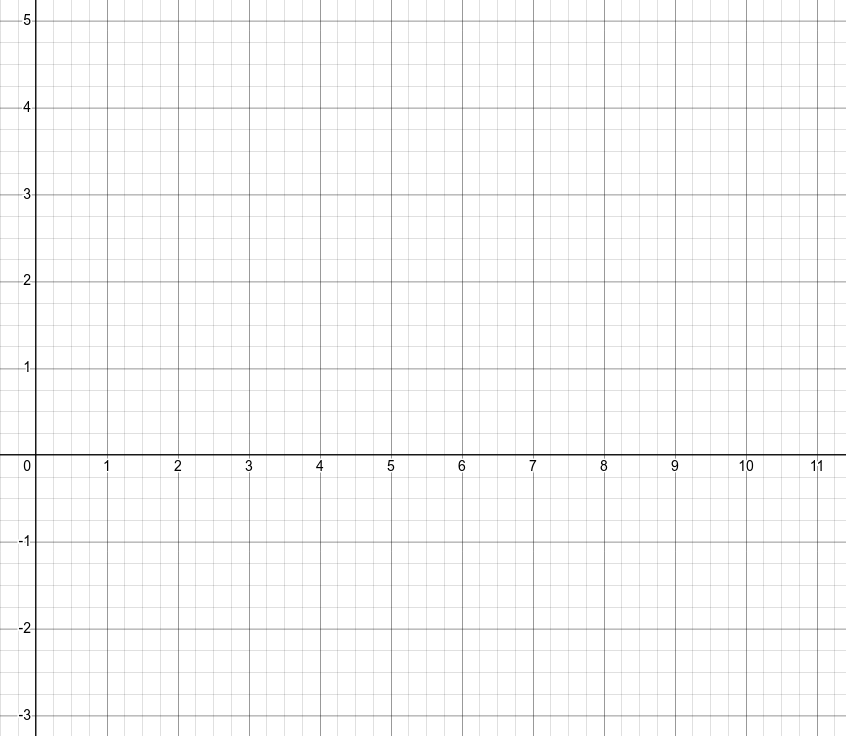
\includegraphics[align = c, width = \textwidth]{StepFunctionAxes}

\end{columns}
\end{frame}
}
%--- Next Frame ---%

%--- Next Frame ---%
\begin{frame}[c]{Step function: Learned model}

\begin{equation*}
	y_i = \beta_0 + \beta_1C_1(x_i) + \beta_2 C_2(x_i) + \cdots + \beta_K C_K(x_i) + \e_i
\end{equation*}
\begin{columns}
\column{.45\textwidth}
\centering
\InstructorList{
	\item Note above we don't learn a coeff for $C_0$ since like qualitative variable version, we can figure out the value from the others.
	\item If $X <c_1$, all predictors are 0 so $\beta_0$ is mean value of $Y$ for $X < c_1$
	\item Then response for $X \in [c_j,c_{j+1})$ is $\beta_0 + \beta_j$, so $\beta_j$ is the avg increase in response for $X$ in the interval relative to $X<c_1$
}


\column{.45\textwidth}
\centering

\end{columns}

\end{frame}
%--- Next Frame ---%

{
\setbeamercolor{background canvas}{bg=Apricot!25}
\begin{frame}[t]{Coding bit}
	Back to the \texttt{wage} data set
\begin{columns}
\column{.45\textwidth}
\centering
\column{.45\textwidth}
\centering
\end{columns}
\end{frame}
}
%--- Next Frame ---%

\begin{frame}[c]{Step function example}

\begin{columns}
\column{.45\textwidth}
\centering
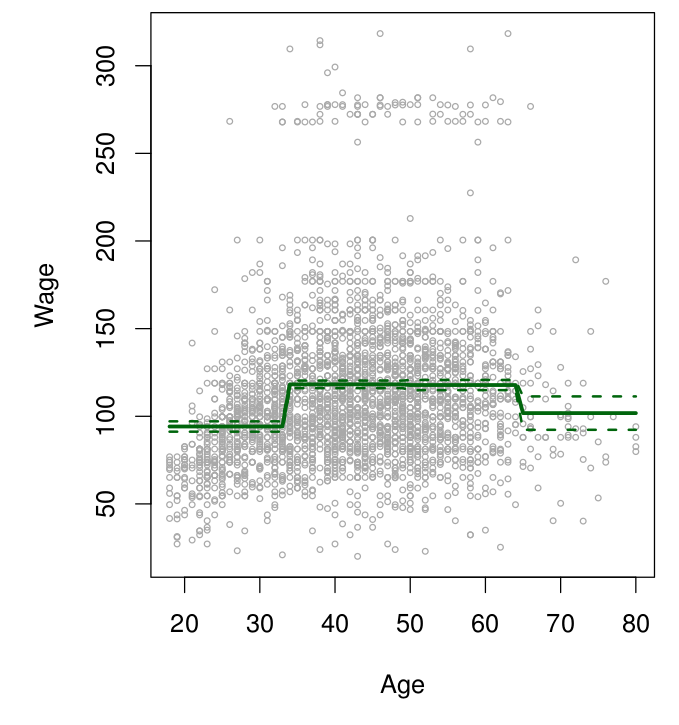
\includegraphics[width = \textwidth, align = c]{Fig7-2a}

\column{.45\textwidth}
\centering
\InstructorList{
  \item Learned peak where the high earners are

}

\end{columns}

\end{frame}
%--- Next Frame ---%

%--- Next Frame ---%


\begin{frame}[t]{Next time}

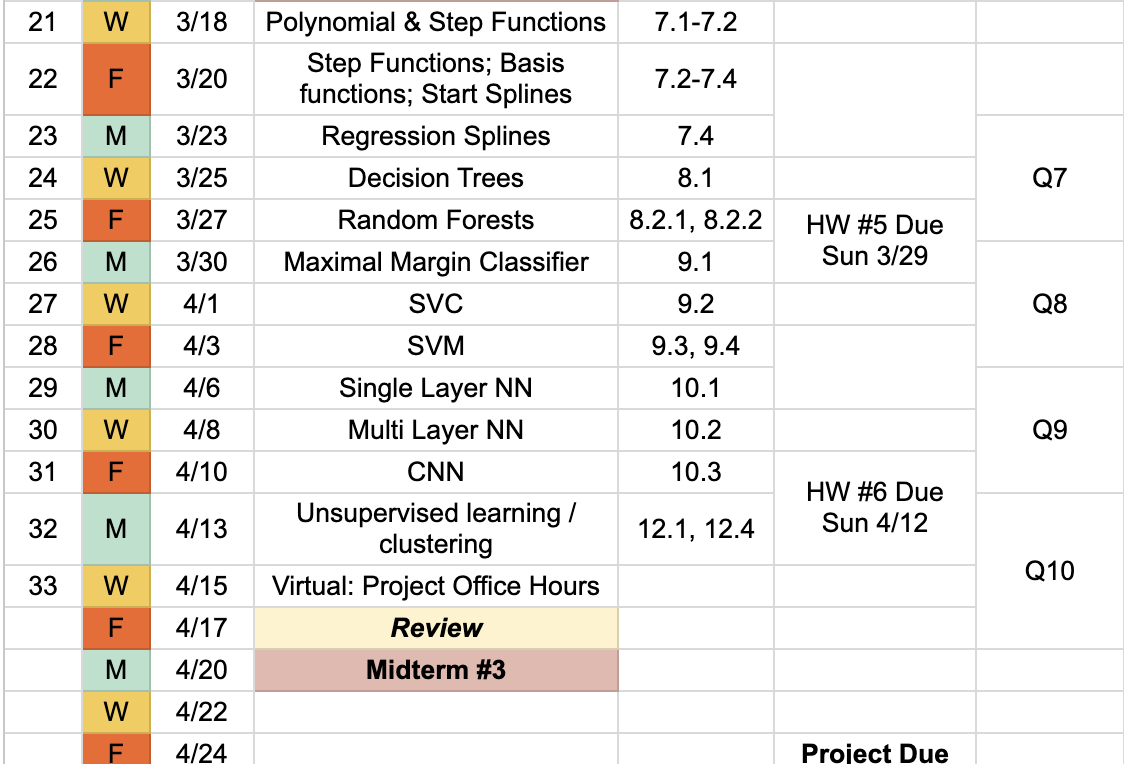
\includegraphics[align = c, width = .45\textwidth]{Schedule-S26-3.png}


\end{frame}
%--- Next Frame ---%


\end{document}
